
\section{Preliminaries}
\label{sec:preliminaries}

Sequence replicated data structures (\emph{sequence} for short) are the closest
structures that can implement a shared document. 

\begin{definition}[Document]
  A document is a series of $k$ characters
  $d(H) = \alpha_1.\alpha_2\ldots \alpha_k$ produced by a series of operations
  $H$.
\end{definition}

\begin{definition}[Replicated sequence]
  Let $d(H)$ the document produced by the series of operations $H$. A replicated
  sequence of $d(H)$ is a structure $r(H)$ with a projection $\pi$ such that
  $\pi(r(H)) \rightarrow d(H)$.
\end{definition}

We focus on replicated sequences~\cite{shapiro2011comprehensive,
  shapiro2011conflict} that provide two commutative operations: \textsc{insert}
and \textsc{delete}. Operations can be integrated in any order as long as the
deletion of an element follows its insertion.

\noindent Each element of the sequence is associated to a unique and immutable
identifier. Using a total order on identifiers, we can project the set of pairs
$\langle element,\, identifier \rangle$ to a sequence of elements. Assuming that
the replicas integrated the same set of operations, they converge to an
identical state, i.e., users see the same document~\cite{shapiro2011conflict}.

Each \textsc{insert} operation generates an identifier for the new element.  For
instance, let us consider a sequence \texttt{QWTY} with the unique, immutable,
and totally ordered integer identifiers $1$, $2$, $4$, and $8$ respectively. A
collaborator inserts \texttt{E} between \texttt{W} and \texttt{T}. The natural
identifier that comes to mind is $3$. The resulting sequence is
\texttt{QWETY}. However, \texttt{R} cannot be inserted between \texttt{E} and
\texttt{T}, for the identifiers $3$ and $4$ are contiguous. The space of
identifiers must be enlarged to handle the new insertion. If we consider
identifiers as decimal numbers, we can associate $3.1$ to the character
\texttt{R}. Since $3 < 3.1 < 4$, the sequence of characters is, as expected,
\texttt{QWERTY}. Inserting a new character between \texttt{E} and \texttt{R}
would result in another space extension : $3.0.X$, where $X$ is an integer.

% If a new character has to be inserted between \texttt{E} and
% \texttt{R}, a new identifier will be allocated between $3$ and $3.1$. Again, the
% space will be extended resulting in a new identifier $3.0$ suffixed by any non
% null integer. Let $X$ be this suffix, the order of the elements of the sequence
% is preserved since $(3 < 3.0.X < 3.1)$.

%% (TODO) are the paths of variable-size identifiers ?
Such growing identifiers are called variable-size identifiers. The main
objective is to keep the growth of the size of the identifiers under a sublinear
boundary.

\subsection{Encoding a position in the sequence}
\label{subsec:variable}

Concatenations of elements (e.g. integers) constitutes a mean to represent
variable-size identifiers.
% can be represented as a concatenation of basic elements (e.g. integers).
A tree structure can represent the resulting sequence. Its nodes store the
elements of the sequence and its edges are labeled such that a path from the
root to a node containing an element represents the main part of the latter's
identifier. For instance, the character $R$ in the previous example is
accessible following the path composed of the edges labeled $3$ then $1$.  This
represents the \emph{path} of an identifier.


% More formally, a sequence is a tree where each node contains a value i.e. an
% element of the sequence (over an alphabet $\mathcal{A}$). The tree is a set of
% pairs $\langle\mathcal{P}\subset\{\mathbb{N}\}^*,\, \mathcal{A} \rangle$, i.e.,
% each element is associated with a path. Additionally, a total order
% ($\mathcal{P}$,$<_{\mathcal{P}}$) provides an ordering among the paths which
% allows to retrieve the order of the elements in the sequence. Notation: a path
% composed of $e$ edges labeled $\ell_1,\ell_2,\ldots,\ell_e$ will be noted
% $[\ell_1.\ell_2\ldots\ell_e]$.

\begin{definition}[Path]
  A path is a series of integers noted $[\ell_1.\ell_2\ldots \ell_e]$ chosen in a
  set $\mathcal{P}$ paired with a dense order $(\mathcal{P},\, <_\mathcal{P})$.
  Each integer $\ell_i$ composing the path is chosen in a set
  $\mathbb{N}_{<X_i}$. The binary representation of a path of size $e$ requires
  $\textstyle \sum\nolimits_{i=1}^e \lceil \log_2 X_i\rceil$ bits.
\end{definition}


\begin{figure*}
  \centering
  \subfloat[The tree is the unions of identifiers.]
  [\label{fig:treemodelexample}The tree representing the sequence is
  built by the union of identifiers and mainly uses paths to order its
  characters.]
  {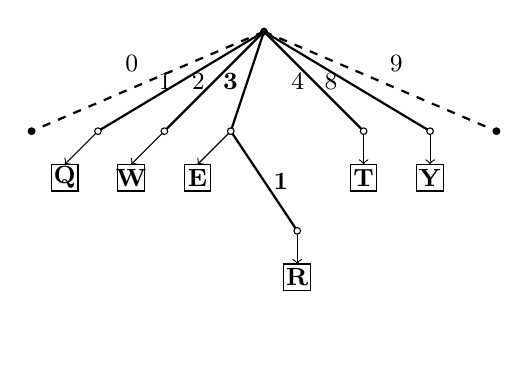
\begin{tikzpicture}[scale=1.2]

\newcommand\Y{-30};
\newcommand\ADDY{-10};

  %% node to node
  \small
  \draw[dashed,thick] (0pt,0pt) -- node[anchor=south east]{0} (-70pt,-30pt);
  \draw[thick] (0pt,0pt) -- node[anchor=east]{1} (-50pt,-30pt); %% Q
  \draw[thick] (0pt,0pt) -- node[anchor=east]{2} (-30pt,-30pt); %% W
  \draw[thick] (0pt,0pt) -- node[anchor=east]{\textbf{3}} (-10pt,-30pt); %% E
  \draw[thick] (0pt,0pt) -- node[anchor=east]{4} ( 30pt,-30pt); %% T
  \draw[thick] (0pt,0pt) -- node[anchor=east]{8} ( 50pt,-30pt); %% Y
  \draw[dashed,thick] (0pt,0pt) -- node[anchor=south west]{9} ( 70pt,-30pt);

  \draw[thick] (-10pt,-30pt) -- node[anchor=west]{\textbf{1}} ( 10pt,-60pt); %% R
%  \draw[thick] (-10pt,-30pt) -- node[anchor=west]{\textbf{0}} (-10pt,-60pt);
%  \draw[thick] (-10pt,-60pt) -- node[anchor=east]{\textbf{X}} (  0pt,-90pt); %% ?


  %% node to element
  \draw[->] (-50pt,\Y pt) -- (-60pt, \ADDY +\Y pt);
  \draw[->] (-30pt,\Y pt) -- (-40pt, \ADDY +\Y pt);
  \draw[->] (-10pt,\Y pt) -- (-20pt, \ADDY +\Y pt);
  \draw[->] ( 30pt,\Y pt) -- ( 30pt, \ADDY +\Y pt);
  \draw[->] ( 50pt,\Y pt) -- ( 50pt, \ADDY +\Y pt);

  \draw[->] ( 10pt,2 * \Y pt) -- ( 10pt, \ADDY + 2 * \Y pt);
%  \draw[->] (  0pt,3 * \Y pt) -- (  0pt, \ADDY + 3 * \Y pt);

  %% nodes
  \draw[fill=black] ( 0pt,  0pt) circle (1pt); 
  \draw[fill=black] (-70pt, -30pt) circle (1pt); 
  \draw[fill=white] (-50pt, -30pt) circle (1pt); %% Q
  \draw[fill=white] (-30pt, -30pt) circle (1pt); %% W
  \draw[fill=white] (-10pt, -30pt) circle (1pt); %% E
  \draw[fill=white] ( 30pt, -30pt) circle (1pt); %% T
  \draw[fill=white] ( 50pt, -30pt) circle (1pt); %% Y
  \draw[fill=black] ( 70pt, -30pt) circle (1pt);

%  \draw[fill=white] (-10pt, 2 * \Y pt) circle (1pt); %% R
  \draw[fill=white] ( 10pt, 2 * \Y pt) circle (1pt); %% x
%  \draw[fill=white] (  0pt, 3 * \Y pt) circle (1pt); %% ?

  %% elements
  \draw[fill=white](-60pt,-4 + \ADDY + \Y pt)
  node{\textbf{Q}} +(-4pt,-4pt) rectangle +(4pt,4pt) ; %% Q
  \draw[fill=white](-40pt,-4 + \ADDY + \Y pt)
  node{\textbf{W}} +(-4pt,-4pt) rectangle +(4pt,4pt) ; %% W
  \draw[fill=white](-20pt,-4 + \ADDY + \Y pt)
  node{\textbf{E}} +(-4pt,-4pt) rectangle +(4pt,4pt) ; %% E
  \draw[fill=white]( 30pt,-4 + \ADDY + \Y pt)
  node{\textbf{T}} +(-4pt,-4pt) rectangle +(4pt,4pt) ; %% T
  \draw[fill=white]( 50pt,-4 + \ADDY + \Y pt)
  node{\textbf{Y}} +(-4pt,-4pt) rectangle +(4pt,4pt) ; %% Y

  \draw[fill=white]( 10pt,-4 + \ADDY + 2 * \Y pt)
  node{\textbf{R}} +(-4pt,-4pt) rectangle +(4pt,4pt) ; %% R
%  \draw[fill=white](  0pt,-4 + \ADDY + 3 * \Y pt)
%  node{\textbf{?}} +(-4pt,-4pt) rectangle +(4pt,4pt) ; %% ?
  \draw(0, -8+\ADDY+ 2.5*\Y pt);

\end{tikzpicture}
}
  \hspace{20pt}
  \subfloat[Disambiguators operate when same paths have been allocated.]
  [\label{fig:disexample}The tree uses disambiguators to maintain an
  equivalent state, even in presence of concurrent insertions resulting
  in same paths. For simplicity sake, only the disambiguators of
  \texttt{E}, \texttt{R}, and \texttt{T} are displayed.]
  {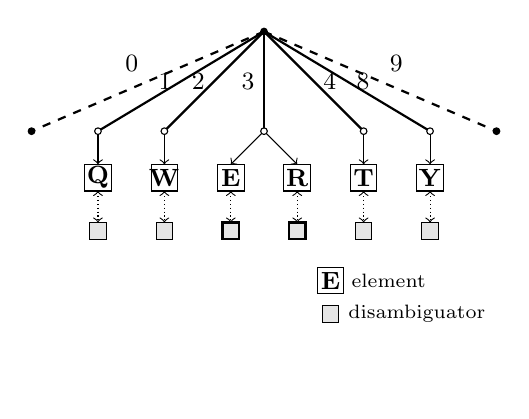
\begin{tikzpicture}[scale=1.2]

\newcommand\Y{-30};
\newcommand\ADDY{-10};

  %% node to node
  \small
  \draw[dashed,thick] (0pt,0pt) -- node[anchor=south east]{0} (-70pt,\Y pt);
  \draw[thick] (0pt,0pt) -- node[anchor=east]{1} (-50pt, \Y pt); %% Q
  \draw[thick] (0pt,0pt) -- node[anchor=east]{2} (-30pt, \Y pt); %% W
  \draw[thick] (0pt,0pt) -- node[anchor=east]{3} (  0pt, \Y pt); %% E R
  \draw[thick] (0pt,0pt) -- node[anchor=west]{4} ( 30pt, \Y pt); %% T
  \draw[thick] (0pt,0pt) -- node[anchor=west]{8} ( 50pt, \Y pt); %% Y
  \draw[dashed,thick] (0pt,0pt) -- node[anchor=south west]{9} ( 70pt, \Y pt);

  %% node to element
  \draw[->] (-50pt,\Y pt) -- (-50pt, \ADDY +\Y pt);
  \draw[->] (-30pt,\Y pt) -- (-30pt, \ADDY +\Y pt);
  \draw[->] (  0pt,\Y pt) -- (-10pt, \ADDY +\Y pt);
  \draw[->] (  0pt,\Y pt) -- ( 10pt, \ADDY +\Y pt);
  \draw[->] ( 30pt,\Y pt) -- ( 30pt, \ADDY +\Y pt);
  \draw[->] ( 50pt,\Y pt) -- ( 50pt, \ADDY +\Y pt);

  %% element to desambiguator
  \draw[<->,densely dotted](-50pt,-8+\ADDY + \Y pt)--(-50pt,2.75*\ADDY+\Y pt);
  \draw[<->,densely dotted](-30pt,-8+\ADDY + \Y pt)--(-30pt,2.75*\ADDY+\Y pt);
  \draw[<->,densely dotted](-10pt,-8+\ADDY + \Y pt)--(-10pt,2.75*\ADDY+\Y pt);
  \draw[<->,densely dotted]( 10pt,-8+\ADDY + \Y pt)--( 10pt,2.75*\ADDY+\Y pt);
  \draw[<->,densely dotted]( 30pt,-8+\ADDY + \Y pt)--( 30pt,2.75*\ADDY+\Y pt);
  \draw[<->,densely dotted]( 50pt,-8+\ADDY + \Y pt)--( 50pt,2.75*\ADDY+\Y pt);

  %% nodes
  \draw[fill=black] ( 0pt, 0 pt) circle (1pt); 
  \draw[fill=black] (-70pt, \Y pt) circle (1pt); 
  \draw[fill=white] (-50pt, \Y pt) circle (1pt); %% Q
  \draw[fill=white] (-30pt, \Y pt) circle (1pt); %% W
  \draw[fill=white] (  0pt, \Y pt) circle (1pt); %% E
  \draw[fill=white] ( 30pt, \Y pt) circle (1pt); %% T
  \draw[fill=white] ( 50pt, \Y pt) circle (1pt); %% Y
  \draw[fill=black] ( 70pt, \Y pt) circle (1pt);

  %% desambiguator
  \draw[fill=gray!20] (-50pt,-2.5+2.75*\ADDY+\Y pt)
  +(-2.5pt,-2.5pt) rectangle +(2.5pt,2.5pt);
  \draw[fill=gray!20] (-30pt,-2.5+2.75*\ADDY+\Y pt)
  +(-2.5pt,-2.5pt) rectangle +(2.5pt,2.5pt);
  \draw[fill=gray!20, thick] (-10pt,-2.5+2.75*\ADDY+\Y pt)
  +(-2.5pt,-2.5pt) rectangle +(2.5pt,2.5pt);
  \draw[fill=gray!20, thick] ( 10pt,-2.5+2.75*\ADDY+\Y pt)
  +(-2.5pt,-2.5pt) rectangle +(2.5pt,2.5pt);
  \draw[fill=gray!20] ( 30pt,-2.5+2.75*\ADDY+\Y pt)
  +(-2.5pt,-2.5pt) rectangle +(2.5pt,2.5pt);
  \draw[fill=gray!20] ( 50pt,-2.5+2.75*\ADDY+\Y pt)
  +(-2.5pt,-2.5pt) rectangle +(2.5pt,2.5pt);

  %% elements
  \draw[fill=white](-50pt,-4 + \ADDY + \Y pt)
  node{\textbf{Q}} +(-4pt,-4pt) rectangle +(4pt,4pt) ; %% Q
  \draw[fill=white](-30pt,-4 + \ADDY + \Y pt)
  node{\textbf{W}} +(-4pt,-4pt) rectangle +(4pt,4pt) ; %% W
  \draw[fill=white](- 10pt,-4 + \ADDY + \Y pt)
  node{\textbf{E}} +(-4pt,-4pt) rectangle +(4pt,4pt) ; %% E
  \draw[fill=white]( 10pt,-4 + \ADDY + \Y pt)
  node{\textbf{R}} +(-4pt,-4pt) rectangle +(4pt,4pt) ; %% R
  \draw[fill=white]( 30pt,-4 + \ADDY + \Y pt)
  node{\textbf{T}} +(-4pt,-4pt) rectangle +(4pt,4pt) ; %% T
  \draw[fill=white]( 50pt,-4 + \ADDY + \Y pt)
  node{\textbf{Y}} +(-4pt,-4pt) rectangle +(4pt,4pt) ; %% Y

  
  \begin{scope}[shift={(20pt, 2.5*\Y pt)}]    
    \draw[fill=white](0,0)node{\textbf{E}} +(-4pt, -4pt) rectangle +(4pt, 4pt);
    \scriptsize
    \draw (4pt, 0)node[anchor=west]{element};
    \draw[fill=gray!20] (0,\ADDY pt) +(-2.5pt, -2.5pt)rectangle+(2.5pt, 2.5pt);
    \draw (3pt, \ADDY pt) node[anchor=west]{disambiguator};
  \end{scope}
  %% spacing
  \draw(0, -8+\ADDY+ 3*\Y pt);

\end{tikzpicture}
}
  \caption{Examples of 10-ary trees containing the sequence of characters
    \texttt{QWERTY}.}
\end{figure*}


Figure~\ref{fig:treemodelexample} shows the underlying 10-ary tree representing
a sequence. Like in the previous scenario, the initial sequence is \texttt{QWTY}
with the respective paths $[1]$, $[2]$, $[4]$ and $[8]$. The insertion of the
character \texttt{E} between the pairs $\langle [2],\, \texttt{W}\rangle$ and
$\langle [4],\, \texttt{T}\rangle$ results in the following pair:
$\langle [3],\, \texttt{E} \rangle$. Then, inserting \texttt{R} between
\texttt{E} and \texttt{T} forces to start a new level, for there is no room at
the first level of the tree for any paths between these bounds. In this example,
the resulting path is $[3.1]$. Using the total order of paths, we retrieve the
sequence \texttt{QWERTY}.
% if label $1$ is chosen for the element \texttt{R}
%at the second level.

\noindent Again, inserting a character between \texttt{E} and \texttt{R} would increase
the depth of the tree.
% in case there is an insertion between the elements
%\texttt{E} and \texttt{R}.
Assuming a 10-ary tree, the new path would be $[3.0.X]$ where $0<X<10$. 



\subsection{Disambiguation of concurrent cases}
\label{subsec:disambiguation}

% Two collaborators concurrently performing an operation on their respective
% replica may get different results after the integration of both
% operations. Indeed,
The order among paths $(\mathcal{P},\,<_\mathcal{P})$ is a total order when a
single collaborator edits. However, it becomes a partial order when the editing
session involves several collaborators and concurrent operations exist. For
instance, two collaborators inserting a character at a same position in the
sequence at a same time may end up with the same allocated path. In such case
the order of characters is not strictly defined and may break the convergence
property. We need a disambiguator in each identifier to preserve a dense total
order among identifiers. This ensures convergent replicas.

%Disambiguators use globally unique markers to provide a total order
%among elements even in presence of concurrent insertions. 

%Each pair of $\langle element,\,path\rangle$ is
%associated with a disambiguator.

\begin{definition}[Disambiguator]
  A disambiguator is a globally unique marker chosen in a set $\mathcal{D}$
  paired with a total order $(\mathcal{D},\, <_\mathcal{D})$. Disambiguators
  usually comprise unique site identifiers along with Lamport
  clocks~\cite{lamport1978time}.
\end{definition}

% Let the set of identifiers $\mathcal{I}$ be the set of unique triples
% $\mathcal{I}:\mathcal{P}\times \mathcal{A}\times \mathcal{D}$. The composition
% of the partial order ($\mathcal{P}$, $<_{\mathcal{P}}$) and the total order of
% disambiguators ($\mathcal{D}$, $<_{\mathcal{D}}$) orders the elements of the
% sequence identically at any replica.

\begin{definition}[Variable-size identifier]
  A variable-size identifier is a triple $\langle p,\, \alpha,\, d \rangle$
  chosen in $\mathcal{I}$ where $p$ is a path chosen in $\mathcal{P}$, $\alpha$
  is an element chosen in an alphabet $\mathcal{A}$, and $d$ is a disambiguator
  chosen in $\mathcal{D}$. The set $\mathcal{I}$ is paired with a dense total
  order $(\mathcal{I},\,<_\mathcal{I})$.
\end{definition}

Figure~\ref{fig:disexample} depicts a tree containing 6 elements with only 5
distinct paths. First, the collaborator $u_1$ inserts \texttt{QW}.  Then, the
collaborators $u_1$ and $u_2$ concurrently insert \texttt{E} and \texttt{T}
respectively. This happens to generate an identical path: [$3$]. To solve any
ambiguity about the order of characters, each identifier includes a
disambiguator.  Let a disambiguator be a series of pairs of unique site
identifiers and counters:
$[\langle s_1,\, c_1 \rangle.\langle s_2,\, c_2 \rangle \ldots \langle s_e,\,
c_e \rangle]$
where $e$ is the size of the path.  The disambiguator
$[\langle u_1,\, 6\rangle]$ is associated with \texttt{E}; the disambiguator
$[\langle u_2,\, 1\rangle]$ is associated with \texttt{T}. The dense total order
is a lexicographic one: at each level we compare the paths, then the site
identifiers, then the counters. It is defined as :
\begin{align*}
  t_i < t_j \iff & (p_i < p_j) \vee \\
                 & ((p_i = p_j) \wedge (s_i<s_j)) \vee \\
                 & ((p_i = p_j) \wedge (s_i = s_j) \wedge (c_i < c_j)) \\
  t_i = t_j \iff & \neg (t_i < t_j) \wedge \neg (t_j < t_i) \\
  id_i <_\mathcal{I} id_j \iff & \exists (m > 0)(\forall n < m),\, (t^i_n = t^j_n) \wedge                             (t^i_m < t^j_m) \\
  id_i =_\mathcal{I} id_j \iff & \forall m,\, t^i_m = t^j_m
\end{align*}
% Retrieving the order of elements simply consists in comparing 
In this example, \texttt{E} precedes \texttt{T} because
$p^\texttt{E}_1=p^\texttt{T}_1$ and $s^\texttt{E}_1 < s^\texttt{T}_1$. Then,
$u_1$ inserts \texttt{Y} at the end of the sequence. Finally, $u_1$ inserts
\texttt{R} between \texttt{E} and \texttt{T}. Since \texttt{E} and \texttt{T}
have an identical path, there is not enough room for new insertions at this
level. The allocation function chooses a path $[3.X]$ where $0<X<10$. By copying
the disambiguator of \texttt{E} at the first level, it ensures that the new
identifier will follow the character \texttt{E} and precede the character
\texttt{T}.

% Collaborators cannot influence the final position of the character in the
% sequence using disambiguators, for disambiguators are automatically computed
% without concerns about positions. The sequence of the example could have ended
% in \texttt{QWTREY} and it would have needed a correction.
%It is worth noting that 
The space complexity of disambiguators is upper-bounded by their respective
path. Therefore, we focus on paths in the rest of the paper.

\subsection{Choosing the smallest path}
\label{subsec:choosing}

The most critical part of sequences with variable-size identifiers consists in
creating the paths. The function that allocates the identifers must provide the
smallest possible paths without impairing future
allocations.

Algorithm~\ref{algo:crdtabstract} shows the general outlines of these
sequences. It divides the operations -- insert and delete -- into the local and
remote parts of the optimistic replication scheme. We can see that the core of
the algorithm and associated complexity lies in the local part of the insert
operation where it generates a path (cf. Line~\ref{line:allocpath}) and a
disambiguator (cf. Line~\ref{line:allocdes}). The function \textsc{convert2Path}
gets rid of the disambiguators of the identifiers in argument to keep paths
only. Without evidence of concurrency, it simply returns the paths contained in
the identifiers. Otherwise, it translates the identifiers into paths that
maintain the order following the order of paths
($\mathcal{P},\, <_{\mathcal{P}}$). For instance in Figure~\ref{fig:disexample},
the result of \textsc{convert2Path} with the identifiers of the character
\texttt{E} and the character \texttt{T} is the pair
$\langle [3.0],\, [3.9]\rangle$. The function \textsc{allocPath} allocates a new
path between these bounds.  \textsc{allocDis} decorates the path in order to
guarantee that the new identifier -- as the composition of a path, an element,
and a disambiguator -- consistently fall between the adjacent identifiers that
served to create it following the order of identifiers
($\mathcal{I}, \, <_\mathcal{I}$).

\begin{algorithm}[h]
  
\small
\algrenewcommand{\algorithmiccomment}[1]{\hskip2em$\rhd$ #1}

\newcommand{\comment}[1]{$\rhd$ #1}


\algblockdefx[initially]{initially}{endInitially}
  [0] {\textbf{INITIALLY:}} 

\algblockdefx[local]{local}{endLocal}
  [0] {\textbf{LOCAL UPDATE:}}

\algblockdefx[received]{received}{endReceived}
  [0] {\textbf{RECEIVED UPDATE:}}

\algblockdefx[onInsert]{onLocal}{endOnLocal}
  [0] {\textbf{on} insert ($p \in \mathcal{I},\,\alpha \in \mathcal{A},\,
   q\in\mathcal{I}$):}
  [0] {\textbf{on} delete ($i \in \mathcal{I}$):} 

\algblockdefx[onRemote]{onRemote}{endOnRemote}
  [0] {\textbf{on} insert ($i\in\mathcal{I}$):\hfill\comment{once per 
  distinct triple in $\mathcal{I}$}}
  [0] {\textbf{on} delete ($i\in\mathcal{I}$):\hfill\comment{after the 
  remote $insert(i)$ is done}} 

\newcommand{\LINEFOR}[2]{%
  \algorithmicfor\ {#1}\ \algorithmicdo\ {#2} %
  }

\newcommand{\LINEIFTHEN}[2]{%
  \algorithmicif\ {#1}\ \algorithmicthen\ {#2} %
  }

\newcommand{\INDSTATE}[1][1]{\State\hspace{\algorithmicindent}}

\begin{algorithmic}[1]
  \Statex
  \initially
    \State $\mathcal{T} \leftarrow \varnothing$; \hfill \comment{structure of
     the CRDT for sequences}
  \endInitially
  
  \local
    \onLocal
    \State \textbf{let} $path \leftarrow allocPath(p.P,\,q.P)$; \label{line:allocpath}
    \State \textbf{let} $dis \leftarrow allocDis(p,\, path,\, q)$; \label{line:allocdes}
    \State $broadcast('insert',\, \langle path,\, \alpha,\, dis \rangle)$;
    \endOnLocal
    \INDSTATE $broadcast('delete',\,i)$;
  \endLocal
  
  \received
    \onRemote
    \State $\mathcal{T} \leftarrow \mathcal{T} \cup i$;
    \endOnRemote
    \INDSTATE $\mathcal{T} \leftarrow \mathcal{T}\, \backslash\, i$; 
  \endReceived
  
\end{algorithmic}

  \caption{\label{algo:crdtabstract}General outlines of a sequence with
    variable-size identifiers.}
\end{algorithm}

The function \textsc{allocPath} chooses a path in the tree between two other paths
$p$ and $q$ where $p$ precedes $q$: $p<_{\mathcal{P}}q$. The new path $n$ must
fall between $p$ and $q$: $p<_\mathcal{P}n<_\mathcal{P}q$.
% However, the number of paths between two paths is infinite, for the order is
% dense, and so is the number of \textsc{allocPath} strategies. Nevertheless,
The function \textsc{allocPath} should choose the smallest available path among all
the possible paths for performance sake.
% This observation reduces considerably the number of possible allocation
% strategies.

\begin{figure*}
  \centering
  \subfloat[Optimal case.]
  [\label{fig:allocpathexampleA} Optimal case.]
  {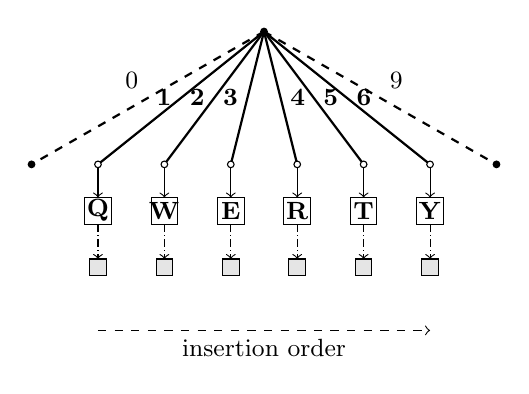
\begin{tikzpicture}[scale=1.2]

  %% node to node
  \small
  \draw[dashed, thick] (0pt,0pt) -- node[anchor=south east]{0} (-70pt,-40pt);
  \draw[thick] (0pt,0pt) -- node[anchor=east]{\textbf{1}} (-50pt,-40pt);
  \draw[thick] (0pt,0pt) -- node[anchor=east]{\textbf{2}} (-30pt,-40pt);
  \draw[thick] (0pt,0pt) -- node[anchor=east]{\textbf{3}} (-10pt,-40pt);
  \draw[thick] (0pt,0pt) -- node[anchor=west]{\textbf{4}} ( 10pt,-40pt);
  \draw[thick] (0pt,0pt) -- node[anchor=west]{\textbf{5}} ( 30pt,-40pt);
  \draw[thick] (0pt,0pt) -- node[anchor=west]{\textbf{6}} ( 50pt,-40pt);
  \draw[dashed, thick] (0pt,0pt) -- node[anchor=south west]{9} ( 70pt,-40pt);

  %% node to element
  \draw[->] (-50pt,-40pt) -- (-50pt,-50pt);
  \draw[->] (-30pt,-40pt) -- (-30pt,-50pt);
  \draw[->] (-10pt,-40pt) -- (-10pt,-50pt);
  \draw[->] ( 10pt,-40pt) -- ( 10pt,-50pt);
  \draw[->] ( 30pt,-40pt) -- ( 30pt,-50pt);
  \draw[->] ( 50pt,-40pt) -- ( 50pt,-50pt);

  %% element to desambiguator
  \draw[->,densely dashdotted] ( -50pt,-58pt) -- ( -50pt,-68.5pt);
  \draw[->,densely dashdotted] ( -30pt,-58pt) -- ( -30pt,-68.5pt);
  \draw[->,densely dashdotted] ( -10pt,-58pt) -- ( -10pt,-68.5pt);
  \draw[->,densely dashdotted] (  10pt,-58pt) -- (  10pt,-68.5pt);
  \draw[->,densely dashdotted] (  30pt,-58pt) -- (  30pt,-68.5pt);
  \draw[->,densely dashdotted] (  50pt,-58pt) -- (  50pt,-68.5pt);

  \draw[fill=black] (  0pt,  0pt) circle (1pt);
  \draw[fill=black] (-70pt,-40pt) circle (1pt);
  \draw[fill=white] (-50pt,-40pt) circle (1pt);
  \draw[fill=white] (-30pt,-40pt) circle (1pt);
  \draw[fill=white] (-10pt,-40pt) circle (1pt);
  \draw[fill=white] ( 10pt,-40pt) circle (1pt);
  \draw[fill=white] ( 30pt,-40pt) circle (1pt);
  \draw[fill=white] ( 50pt,-40pt) circle (1pt);
  \draw[fill=black] ( 70pt,-40pt) circle (1pt);

  %% elements
  \draw[fill=white](-50pt,-54pt)
  node{\textbf{Q}}+(-4pt,-4pt)rectangle+(4pt,4pt) ;
  \draw[fill=white](50pt,-54pt)
  node{\textbf{Y}} +(-4pt,-4pt) rectangle +(4pt,4pt) ;
  \draw[fill=white]( 10pt,-54pt)
  node{\textbf{R}} +(-4pt,-4pt) rectangle +(4pt,4pt) ;
  \draw[fill=white] ( -30pt,-54pt)
  node{\textbf{W}} +(-4pt,-4pt) rectangle +(4pt,4pt) ;
  \draw[fill=white] ( -10pt,-54pt)
  node{\textbf{E}} +(-4pt,-4pt) rectangle +(4pt,4pt) ;
  \draw[fill=white]( 30pt,-54pt)
  node{\textbf{T}} +(-4pt,-4pt) rectangle +(4pt,4pt) ;

  %% desambiguator
  \draw[fill=gray!20] (-50pt,-71pt) +(-2.5pt,-2.5pt) rectangle +(2.5pt,2.5pt);
  \draw[fill=gray!20] (-30pt,-71pt) +(-2.5pt,-2.5pt) rectangle +(2.5pt,2.5pt);
  \draw[fill=gray!20] (-10pt,-71pt) +(-2.5pt,-2.5pt) rectangle +(2.5pt,2.5pt);
  \draw[fill=gray!20] ( 10pt,-71pt) +(-2.5pt,-2.5pt) rectangle +(2.5pt,2.5pt);
  \draw[fill=gray!20] ( 30pt,-71pt) +(-2.5pt,-2.5pt) rectangle +(2.5pt,2.5pt);
  \draw[fill=gray!20] ( 50pt,-71pt) +(-2.5pt,-2.5pt) rectangle +(2.5pt,2.5pt);

  %% insertion order
  \draw[->,dashed] (-50pt, -90pt) -- node[anchor=north]{insertion order}
  (50pt, -90pt);

\end{tikzpicture}
}
  \hspace{50pt}
  \subfloat[Worst case.]
  [\label{fig:allocpathexampleB} Worst case.]
  {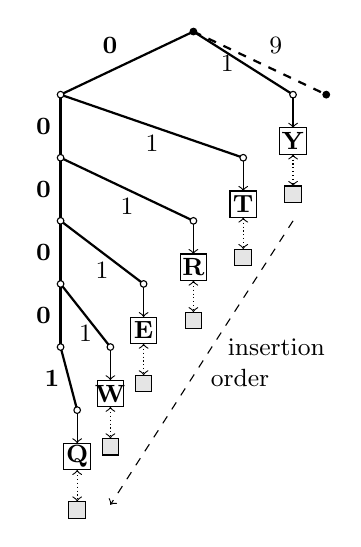
\begin{tikzpicture}[scale=1.2]

\newcommand\Y{-19}
\newcommand\ADDY{-10}

  %% node to node
  \small
  \draw[thick] (0pt,0pt) -- node[anchor=south east]{\textbf{0}} (-40pt,\Y pt);
  \draw[thick] (0pt,0pt) -- node[anchor=east]{1} (30pt, \Y pt); %% Y
  \draw[thick] (-40pt, \Y pt) -- node[anchor=north]{1} (15pt, 2 * \Y pt); %% T
  \draw[thick] (-40pt, \Y pt) -- node[anchor=east]{\textbf{0}} (-40pt, 2 * \Y pt); %% 0
  \draw[thick] (-40pt, 2*\Y pt) -- node[anchor=north]{1} (0pt, 3 * \Y pt); %% R
  \draw[thick] (-40pt, 2*\Y pt)-- node[anchor=east]{\textbf{0}}(-40pt, 3 * \Y pt); %% 0
  \draw[thick] (-40pt, 3*\Y pt) -- node[anchor=north]{1}(-15pt,4 * \Y pt); %% E
  \draw[thick] (-40pt, 3*\Y pt) -- node[anchor=east]{\textbf{0}}(-40pt,4 * \Y pt); %% 0
  \draw[thick] (-40pt, 4*\Y pt) -- node[anchor=north]{1}(-25pt,5 * \Y pt); %% W
  \draw[thick] (-40pt, 4*\Y pt) -- node[anchor=east]{\textbf{0}}(-40pt,5 * \Y pt); %% 0
  \draw[thick] (-40pt, 5*\Y pt) -- node[anchor=east]{\textbf{1}}(-35pt,6 * \Y pt); %% Q

  \draw[dashed, thick] (0pt,0pt) -- node[anchor=south west]{9} (40pt,\Y pt);

  %% node to element
  \draw[->] ( 30pt, \Y pt) -- ( 30pt, \ADDY + \Y pt); %% Y
  \draw[->] ( 15pt, 2* \Y pt) -- ( 15pt, \ADDY + 2 *\Y pt); %% T
  \draw[->] (  0pt, 3 *\Y pt) -- (  0pt, \ADDY + 3 *\Y pt); %% R
  \draw[->] (-15pt, 4 *\Y pt) -- ( -15pt, \ADDY + 4 *\Y pt); %% E
  \draw[->] (-25pt, 5 *\Y pt) -- ( -25pt, \ADDY + 5 *\Y pt); %% W
  \draw[->] (-35pt, 6 *\Y pt) -- ( -35pt, \ADDY + 6 *\Y pt); %% Q

  %% element to desambiguator
  \draw[<->,densely dotted]
  ( 30pt,-8+ \ADDY + \Y pt) -- ( 30pt,2.75*\ADDY+\Y pt); %% Y
  \draw[<->,densely dotted]
  ( 15pt,-8+ \ADDY + 2* \Y pt) -- ( 15pt,2.75*\ADDY+ 2* \Y pt); %% T
  \draw[<->,densely dotted]
  ( 0pt,-8+ \ADDY + 3* \Y pt) -- (  0pt,2.75*\ADDY+ 3* \Y pt); %% R
  \draw[<->,densely dotted]
  ( -15pt,-8+ \ADDY + 4 *\Y pt) -- ( -15pt,2.75*\ADDY+ 4* \Y pt); %% E
  \draw[<->,densely dotted]
  ( -25pt,-8+ \ADDY + 5 *\Y pt) -- ( -25pt,2.75*\ADDY+ 5*\Y pt); %% W
  \draw[<->,densely dotted]
  ( -35pt,-8+ \ADDY + 6* \Y pt) -- ( -35pt,2.75*\ADDY+ 6*\Y pt); %% Q

  %% node
  \draw[fill=black] (0pt,0pt) circle (1pt); %% rooot
  \draw[fill=white] ( 30pt, \Y pt) circle (1pt); %% Y
  \draw[fill=white] (-40pt, \Y pt) circle (1pt); %% 0
  \draw[fill=white] ( 15 pt, 2 * \Y pt) circle (1pt); %% T
  \draw[fill=white] (-40pt, 2 * \Y pt) circle (1pt); %% 0
  \draw[fill=white] (  0 pt, 3 * \Y pt) circle (1pt); %% R
  \draw[fill=white] (-40pt, 3 * \Y pt) circle (1pt); %% 0
  \draw[fill=white] (-15 pt, 4 * \Y pt) circle (1pt); %% E
  \draw[fill=white] (-40pt, 4 * \Y pt) circle (1pt); %% 0
  \draw[fill=white] (-25 pt, 5 * \Y pt) circle (1pt); %% W
  \draw[fill=white] (-40pt, 5 * \Y pt) circle (1pt); %% 0
  \draw[fill=white] (-35 pt, 6 * \Y pt) circle (1pt); %% Q

  \draw[fill=black] ( 40pt, \Y pt) circle (1pt);


  %% elements
  \draw[fill=white] ( 30pt, -4 + \ADDY + \Y pt)
  node{\textbf{Y}} +(-4pt,-4pt) rectangle +(4pt,4pt) ; %% Y
  \draw[fill=white] ( 15pt, -4 + \ADDY +  2 *\Y pt)
  node{\textbf{T}} +(-4pt,-4pt) rectangle +(4pt,4pt) ; %% T
  \draw[fill=white] (  0pt, -4 + \ADDY +  3* \Y pt)
  node{\textbf{R}} +(-4pt,-4pt) rectangle +(4pt,4pt) ; %% R
  \draw[fill=white] (-15pt, -4 + \ADDY + 4 *\Y pt)
  node{\textbf{E}} +(-4pt,-4pt) rectangle +(4pt,4pt) ; %% E
  \draw[fill=white] (-25pt, -4 + \ADDY + 5 * \Y pt)
  node{\textbf{W}} +(-4pt,-4pt) rectangle +(4pt,4pt) ; %% W
  \draw[fill=white] (-35pt, -4 + \ADDY + 6 *\Y pt)
  node{\textbf{Q}} +(-4pt,-4pt) rectangle +(4pt,4pt) ; %% Q

  %% desambiguator
  \draw[fill=gray!20]( 30pt, -2.5 + 2.75 * \ADDY + \Y pt)
  +(-2.5pt,-2.5pt) rectangle +(2.5pt,2.5pt);
  \draw[fill=gray!20]( 15pt, -2.5 + 2.75 * \ADDY +2 *\Y pt)
  +(-2.5pt,-2.5pt) rectangle +(2.5pt,2.5pt);
  \draw[fill=gray!20](  0pt, -2.5 + 2.75 * \ADDY + 3*\Y pt)
  +(-2.5pt,-2.5pt) rectangle +(2.5pt,2.5pt);
  \draw[fill=gray!20](-15pt, -2.5 + 2.75 * \ADDY +4*\Y pt )
  +(-2.5pt,-2.5pt) rectangle +(2.5pt,2.5pt);
  \draw[fill=gray!20](-25pt, -2.5 + 2.75 * \ADDY + 5*\Y pt)
  +(-2.5pt,-2.5pt) rectangle +(2.5pt,2.5pt);
  \draw[fill=gray!20](-35pt, -2.5 + 2.75 * \ADDY +6*\Y pt) 
  +(-2.5pt,-2.5pt) rectangle +(2.5pt,2.5pt);

  %% insertion order
  \draw[->,dashed] (30pt, 3 * \Y pt) -- node[anchor=west,align=left]
  {\ \ insertion\\ order} (-25pt, 7.5 * \Y pt);

\end{tikzpicture}
}
  \caption{\label{fig:allocpathexample} Two trees filled with the resulting
    identifiers of two different permutations resulting in an identical sequence
    \texttt{QWERTY}. The function \textsc{allocPath} allocates the leftmost
    branch in the tree. All paths of the optimal case have a length of 1 while
    the tree of the worst case grows up to a depth of 6.}
\end{figure*}

As illustrated in Figure~\ref{fig:allocpathexample}, the allocation of paths
without an \emph{a priori} knowledge of the final sequence is a non-trivial
problem.  Suppose that \textsc{allocPath} allocates the leftmost branch
available at the lowest depth possible. Suppose two insertion orders resulting
in an identical sequence of characters \texttt{QWERTY}.  In the first case,
\texttt{Q} is inserted first at position 0, followed by \texttt{W} at position 1
(after \texttt{Q}) then \texttt{E} is inserted at position 3 (after \texttt{W}),
etc.  In the second case, \texttt{Y} is inserted first at position 0 as the
sequence is initially empty. Then \texttt{T} is inserted. However as the final
intended word is \texttt{QWERTY}, \texttt{T} has to be inserted at a position
before \texttt{Y} that represents the current state of the sequence. \texttt{T}
is thus inserted at position 0 shifting \texttt{Y} to position 1, etc.


\begin{itemize}[noitemsep, leftmargin=*]
\item Figure~\ref{fig:allocpathexampleA}: In this case, the insertion order
  exactly follows the expectations of the allocation function. The depth of the
  tree never grows. The execution of operations remain efficient.

\item Figure~\ref{fig:allocpathexampleB}: In this case, the insertion order goes
  against the expectations of the allocation function. The depth of the tree
  increase at each insertion. Indeed, as an element gets the smallest value at
  its level, there is no room for a new element at the same level, hence the
  creation of a new level. The depth of the tree grows very fast decreasing the
  efficiency of operations.
\end{itemize}

This example shows how the insertion order impacts the length of the allocated
paths. Unfortunately, the insertion order cannot be predicted, nor the size of
the final sequence. Prior work on sequences often made the assumption of a
left-to-right editing due to observations made on
corpora~\cite{preguica2009commutative, weiss2009logoot}. However, there exist
human edited documents that do not correspond to this kind of
editing~\cite{nedelec2013lseq}.
%% Indeed, the editing depends on the type of the document and to the activity
%% for example when correcting a document the editing in mainly random as the
%% insertions and deletions corresponds to errors distributed in the document.
Hence the need of an allocation function which provides identifiers with a
sublinear space complexity compared to the number of insertions whatever is the
editing sequence. Such allocation function would avoid the need for consensus
algorithm~\cite{mostefaoui2015signature} and would make CRDT-based editors a
practicable alternative to the current mainstream editors.

\begin{problem}
  Let $s(I)= id_1.id_2\ldots id_I$ be the sequence of identifiers, and
  $s(I+1) = s(I) \cup \textsc{insert}(p,\, \_,\, n)$, with $p,q \in s(I)$ and
  $p<_\mathcal{I}q$. Let $|s(I)|$ be the size of the binary representation of
  the sequence. The function \textsc{insert} must allocate identifiers such
  that:
  \begin{equation}
    |s(I+1)| - |s(I)| < \mathcal{O}(I)
  \end{equation}
\end{problem}

 
%%% Local Variables:
%%% mode: latex
%%% TeX-master: "../paper"
%%% End:
